\documentclass{beamer}
\usepackage[utf8]{inputenc}
\usepackage[export]{adjustbox}
\usepackage{hyperref}
\hypersetup{
	colorlinks=true,
	urlcolor=adcorange,
	linkcolor=adcblue
}

\usetheme{Madrid}

\title{Hugo website builder workshop!}
\subtitle{Make a portfolio website!}
\author{Nathaniel Budijono}
\date{April 26, 2022}
\institute{UMN ADC}

\definecolor{adcblue}{RGB}{115,203,255}
\definecolor{adcorange}{RGB}{242,114,0}

\setbeamercolor{palette primary}{fg=white,bg=adcblue}
\setbeamercolor{palette secondary}{fg=adcorange,bg=white}
\setbeamercolor{structure}{fg=adcblue,bg=white}
\setbeamercolor{title in head/foot}{fg=adcblue,bg=white}
\setbeamercolor{date in head/foot}{fg=gray,bg=white}
\setbeamercolor{palette tertiary}{fg=white,bg=adcorange}

\begin{document}

\begin{frame}
    \titlepage
    \includegraphics[width=0.25\textwidth, right]{figs/ADC_Logo_Blue.png}
\end{frame}

\begin{frame}{What is Hugo?}
	\centering
	
\includegraphics[width=0.5\textwidth]{figs/hugo.png}
\end{frame}

\begin{frame}{What is GitHub Pages?}
	\centering
	
\includegraphics[width=0.25\textwidth]{figs/gh-pages.png}
\end{frame}

\begin{frame}{Hugo/GH Pages powers the ADC website}
	\centering
	
\includegraphics[width=0.6\textwidth]{figs/adc-website.png}
	\bigbreak
	\href{https://adcumn.org}{https://adcumn.org}
\end{frame}

\begin{frame}{Setup}
	\begin{enumerate}
		\item \href{https://github.com/join}{Create a GitHub account} \pause
		\item \href{https://git-scm.com/downloads}{Install git} \pause
		\item \href{https://gohugo.io/getting-started/installing/}{Install Hugo} \pause
		\item \href{https://themes.gohugo.io/tags/portfolio/}{Pick a theme}
	\end{enumerate}
\end{frame}

\begin{frame}{Theme-agnostic tips}
	\begin{itemize}
		\item Read your theme's documentation! It may also have an \texttt{exampleSite} directory in its GitHub repo. See its \texttt{config.toml}. \pause
		\item Running \texttt{hugo new site <your-site-name>} makes a new directory called \texttt{<your-sitename>} with subdirectories called \texttt{content}, \texttt{static}, and \texttt{themes}. \pause
		\item Clone your theme's GitHub repo into \texttt{themes}. \pause
		\item \texttt{hugo new <title>.md} creates a new page \texttt{<title>.md} in the \texttt{content} folder and autogenerates the front matter. \pause
		\item See the \href{https://github.com/adam-p/markdown-here/wiki/Markdown-Cheatsheet}{Markdown cheat sheet}. \pause
		\item Run the website locally with \texttt{hugo server} and view at \texttt{localhost:1313}.
	\end{itemize}
\end{frame}

\begin{frame}{Creating a Toha site}
	\href{https://themes.gohugo.io/toha/}{Toha theme} \pause
	\bigbreak
	\begin{enumerate}
		\item Clone the starter code: \texttt{git clone --recurse-submodules https://github.com/hugo-toha/hugo-toha.github.io} \pause
		\item Run the website locally
	\end{enumerate}
\end{frame}

\begin{frame}{Deploying the site (first time)}
	\centering
	
\includegraphics[width=0.5\textwidth]{figs/settings.png}
	\bigbreak
	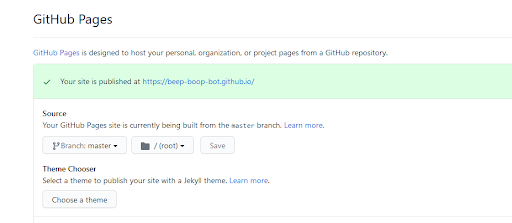
\includegraphics[width=0.5\textwidth]{figs/activate-ghp.png}
	\bigbreak
	\texttt{git submodule add -b main https://github.com/<your-username>/<your-username>.github.io.git public}
	\bigbreak
	\texttt{hugo}
\end{frame}

\begin{frame}{Deploying the site (each update)}
	\begin{enumerate}
		\item Log changes to git: \texttt{git add .} \pause
		\item Commit changes: \texttt{git commit -m "a descriptive message"} \pause
		\item Push changes to GitHub: \texttt{git push -u origin master}
	\end{enumerate}
\end{frame}

\end{document}